\documentclass[12pt,addpoints]{repaso}
\grado{2}
\nivel{Secundaria}
\cicloescolar{2023-2024}
\materia{Ciencias y Tecnología: Física}
\unidad{3}
\title{Practica la Unidad}
\aprendizajes{
\item Describe la generación, diversidad y comportamiento de las ondas
    electromagnéticas como resultado de la interacción entre electricidad y
    magnetismo.
    \item Describe cómo se lleva a cabo la exploración de los cuerpos
    celestes por medio de la detección de las ondas electromagnéticas que emiten.
    \item Describe algunos avances en las características y composición del
    Universo (estrellas, galaxias y otros sistemas).
    \item Describe las características y dinámica del Sistema Solar.
    \item Identifica algunos aspectos sobre la evolución del Universo.
    }
\author{Melchor Pinto, J.C.}
\begin{document}
\INFO%
\begin{multicols}{2}%
     \include*{../blocks/block006b}
     \include*{../blocks/block006c}
\end{multicols}%
\begin{questions}
     \questionboxed[10]{\include*{../questions/question087a}}
     \questionboxed[10]{\include*{../questions/question086a}}
     \ejemplosboxed[\include*{../questions/question076aa}]
     \questionboxed[10]{\include*{../questions/question076a}}
     \questionboxed[10]{\include*{../questions/question076aaa}}
     \questionboxed[10]{\include*{../questions/question079b}}
     \questionboxed[10]{\include*{../questions/question090a}}
     \questionboxed[10]{\include*{../questions/question085d}}
     \questionboxed[10]{\include*{../questions/question088b}}
     \questionboxed[10]{\include*{../questions/question087c}}
     \questionboxed[10]{\include*{../questions/question089b}}
     \questionboxed[6]{Indica si las siguientes afrirmaciones son falsas o verdaderas:

          \begin{multicols}{2}
               \begin{parts}

                    \part La fuerza magnética es una interacción de acción a distancia, también llamada fuerza de campo.

                    \begin{oneparchoices}
                         \choice Verdadero
                         \choice Falso
                    \end{oneparchoices}

                    \part La Tierra posee un campo magnético debido a las corrientes internas en su núcleo de hierro fundido.

                    \begin{oneparchoices}
                         \choice Verdadero
                         \choice Falso
                    \end{oneparchoices}

                    \part Cuando acercamos dos imanes por sus polos iguales, los campos magnéticos interactúan y se suman, de tal forma que los imanes experimentan una fuerza de atracción mutua.

                    \begin{oneparchoices}
                         \choice Verdadero
                         \choice Falso
                    \end{oneparchoices}

                    \part En la siguiente imagen se puede apreciar, mediante el ordenamiento de las limaduras de hierro, el campo magnético de los polos iguales de dos imanes.

                    \begin{oneparchoices}
                         \choice Verdadero
                         \choice Falso
                    \end{oneparchoices}\hfill
                    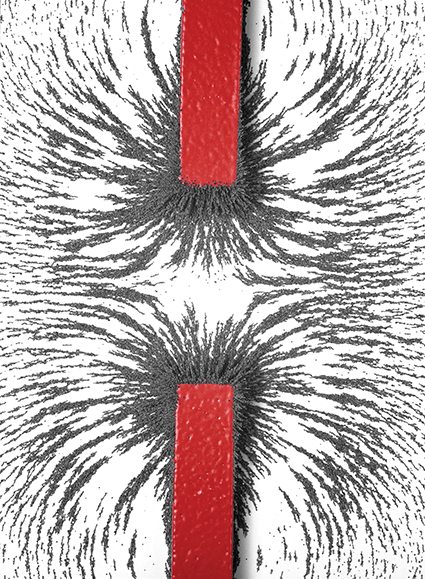
\includegraphics[width=0.3\linewidth]{SINFI_U2_AC67_IMGS4.jpg}

                    \part Sólo las cargas masivas producen campos magnéticos.

                    \begin{oneparchoices}
                         \choice Verdadero
                         \choice Falso
                    \end{oneparchoices}

                    \part Toda carga en movimiento genera un campo magnético.

                    \begin{oneparchoices}
                         \choice Verdadero
                         \choice Falso
                    \end{oneparchoices}

                    \part Los electrones que orbitan alrededor del núcleo generan corrientes eléctricas que, a su vez, producen campos magnéticos, por lo que los átomos se comportan como imanes.

                    \begin{oneparchoices}
                         \choice Verdadero
                         \choice Falso
                    \end{oneparchoices}

                    \part En la siguiente figura, la flecha azul indica la dirección del campo magnético.
                    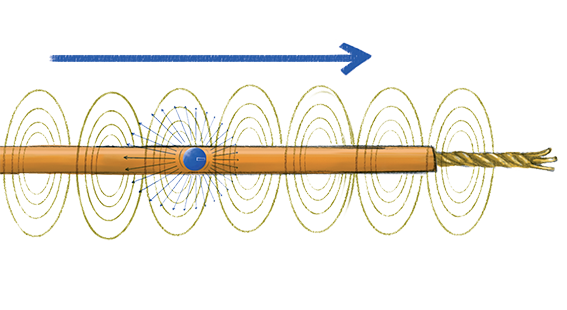
\includegraphics[width=\linewidth]{SINFI_U2_AC67_IMGS2.png}
                    \begin{oneparchoices}
                         \choice Verdadero
                         \choice Falso
                    \end{oneparchoices}\hfill


                    \part La siguiente figura ilustra el ordenamiento de los “imanes atómicos” de un material magnético.

                    \begin{oneparchoices}
                         \choice Verdadero
                         \choice Falso
                    \end{oneparchoices}\hfill
                    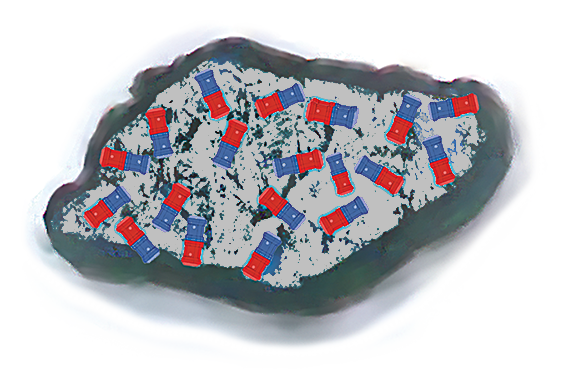
\includegraphics[width=0.4\linewidth]{SINFI_U2_AC67_IMGS3.png}


                    \part La dirección del campo magnético de un conductor largo y recto por el que circula una corriente es circular y rodea al alambre.

                    \begin{oneparchoices}
                         \choice Verdadero
                         \choice Falso
                    \end{oneparchoices}


               \end{parts}
          \end{multicols}
     }
\end{questions}
\end{document}
